%versi 2 (8-10-2016) 
\chapter{Pendahuluan}
\label{chap:intro}
   
\section{Latar Belakang}
\label{sec:label}

Sebuah lokasi atau titik geografis yang memiliki kegunaan tertentu biasa disebut sebagai \textit{Point of interest} (POI). POI ini dapat berupa tempat apa saja yang memiliki ciri khas tertentu dan dapat dikenali dari ciri khas tersebut. POI-POI tertentu dapat dikenali dari logo tempat tersebut atau objek-objek lainnya yang terlihat secara langsung. Seperti ditunjukkan pada Gambar~\ref{fig:poi_with_logo}, kedua POI tersebut memiliki logo unik yang terlihat dengan jelas.

Pada skripsi ini akan dibuat sebuah sistem untuk mengidentifikasi POI dari masukan yang berisi gambar POI tersebut. Proses identifikasi POI dilakukan dengan mendeteksi logo khusus atau objek unik yang ada pada POI tersebut.
\begin{figure}[H]
	\centering
	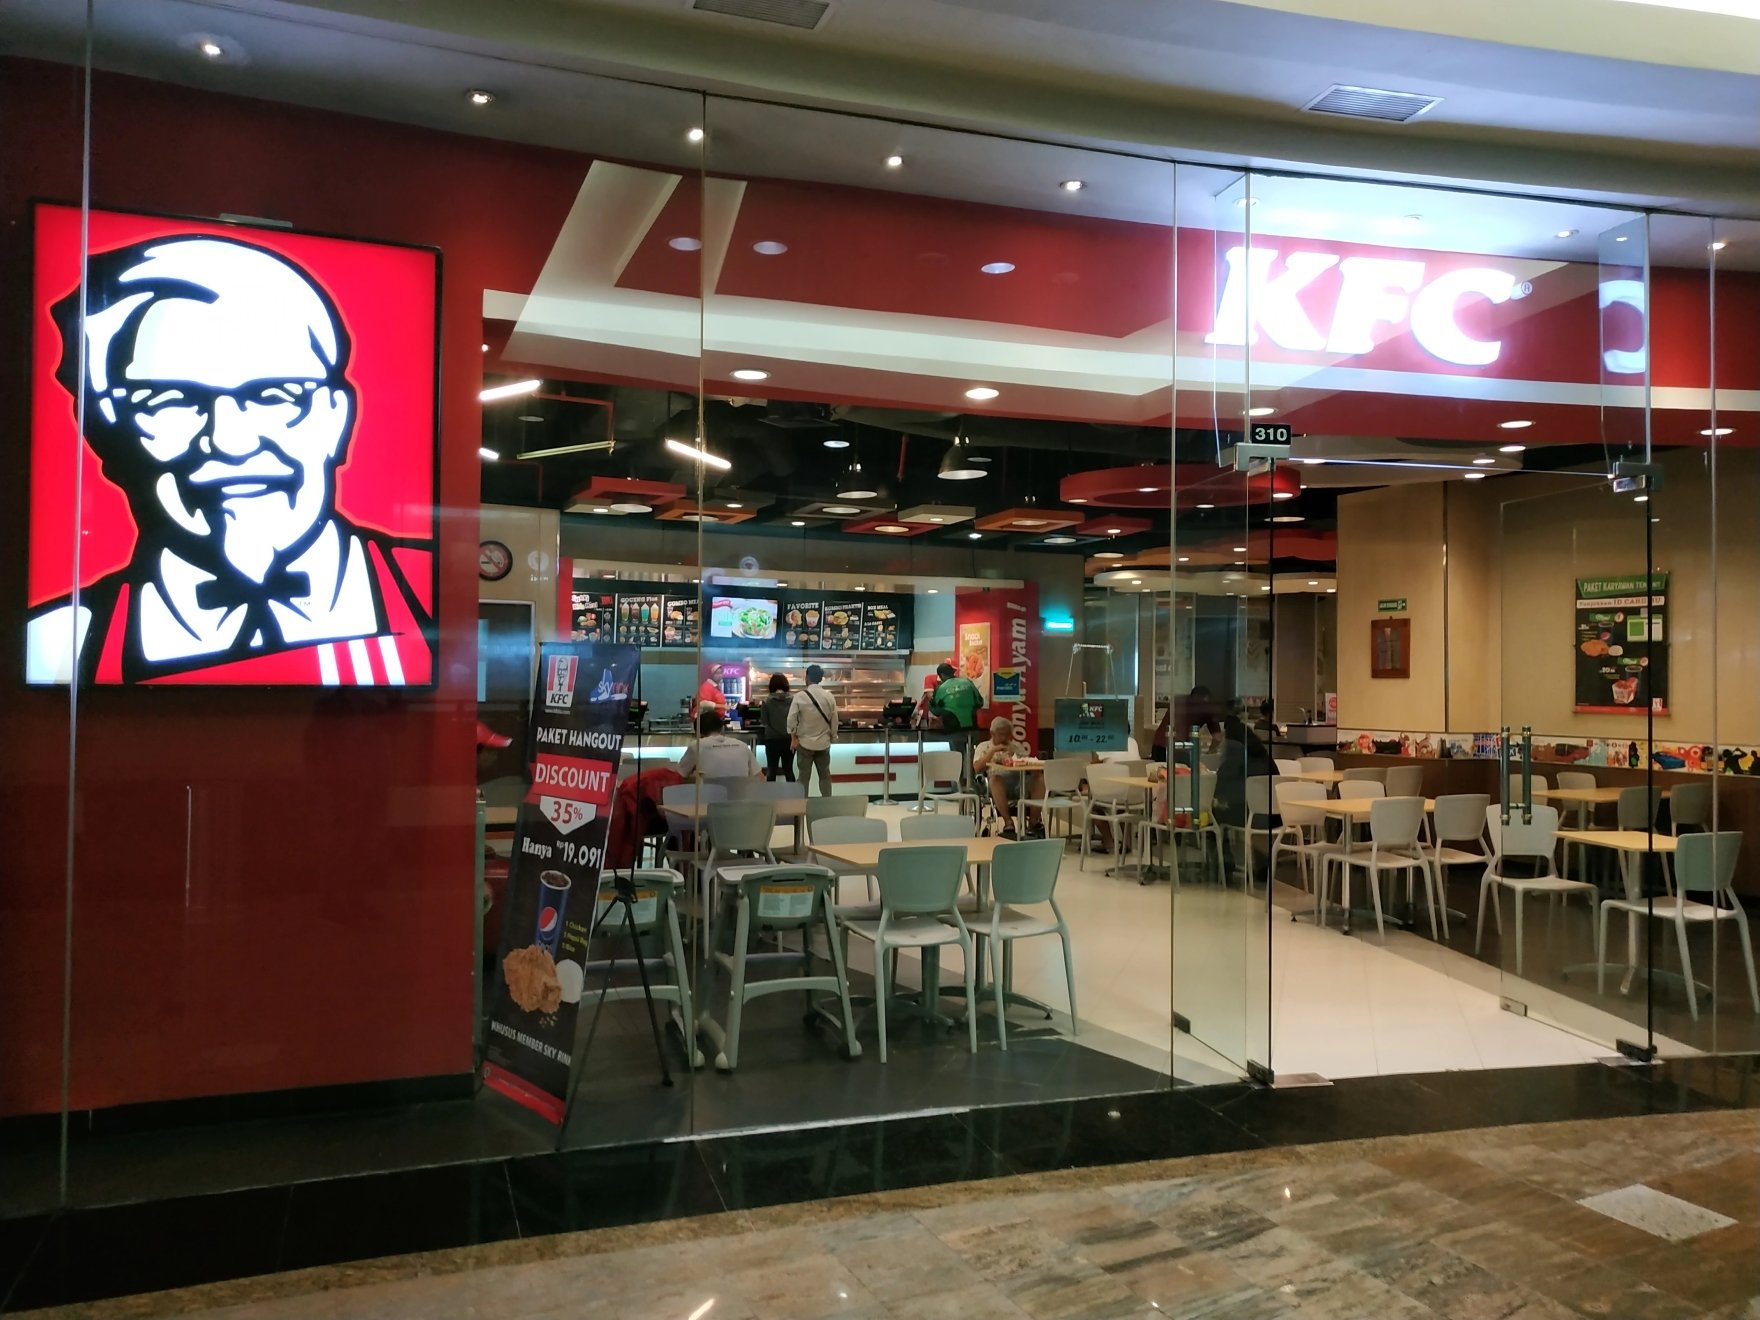
\includegraphics[width=0.4\linewidth]{kfc.jpg}
	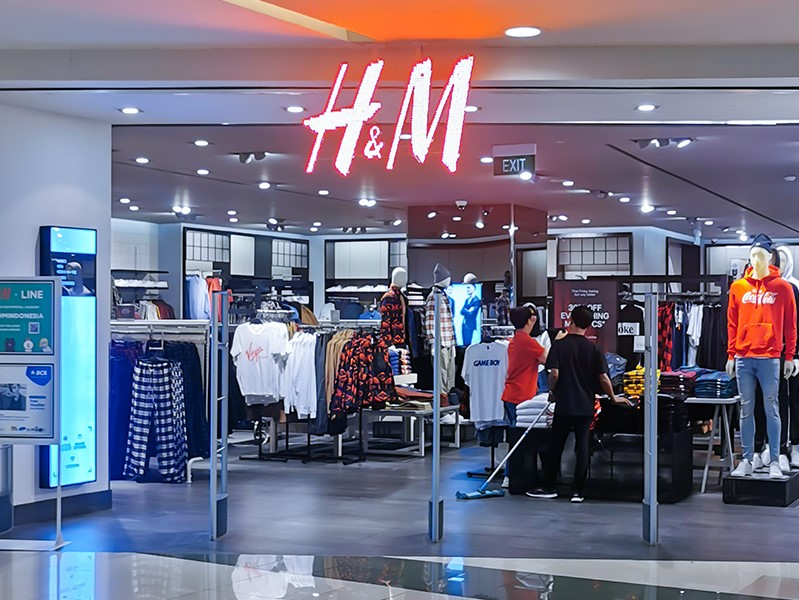
\includegraphics[width=0.4\linewidth]{HM-photo.jpg}
	\caption{Contoh POI yang memiliki logo unik. POI seperti ini dapat dikenali dengan melakukan identifikasi pada logo tersebut.}
	\label{fig:poi_with_logo}
\end{figure}

Proses identifikasi POI akan dilakukan menggunakan teknik \textit{Object Instance Recognition} (OIR). Teknik OIR merupakan teknik pengenalan objek spesifik. Sebuah algoritma OIR harus dapat mengatasi masalah seperti pencahayaan, sudut pengambilan, objek \textit{background}. Objek harus tetap dapat diidentifikasi walaupun gambar memiliki gangguan-gangguan tersebut. OIR dapat dilakukan dengan memanfaatkan fitur lokal.

Fitur lokal merupakan fitur yang mendeskripsikan sebuah daerah penting (\textit{keypoint}) pada gambar. Salah satu cara mendapatkan \textit{Keypoint} adalah dengan mencari sudut-sudut atau perpotongan garis yang terdapat pada gambar. \textit{Keypoint-keypoint} yang terdeteksi pada gambar akan memiliki sebuah vektor untuk mendeskripsikan daerah di sekitar \textit{keypoint} tersebut yang disebut sebagai vektor deskriptor. Proses pencarian fitur lokal pada penelitian ini akan dilakukan dengan menggunakan metode \textit{Scale Invariant Feature Transform} (SIFT) dan \textit{Oriented FAST and Rotated BRIEF} (ORB). Metode SIFT dan ORB akan menghasilkan vektor deskriptor untuk tiap fitur lokal yang terdeteksi, vektor deskriptor ini dapat digunakan untuk mengidentifikasi fitur lokal.

Salah satu masalah yang ada pada pengenalan POI adalah pada sebuah gambar POI tidak semua fitur lokal yang dideteksi bersifat unik terhadap POI tersebut. Ada fitur lokal yang juga dimiliki oleh POI lain atau fitur lokal yang berasal dari objek di latar belakang yang sifatnya tidak konsisten. Masalah ini akan mempersulit pada proses OIR untuk mengidentifikasi POI yang tepat. Gambar~\ref{fig:keypoint_non_unique} menunjukkan masalah-masalah ini, gambar \ref{subfig:audi} dan \ref{subfig:chanel} menunjukkan fitur lokal yang mirip dari dua POI yang berbeda, sedangkan gambar \ref{subfig:cgv} dan \ref{subfig:cgv2} menunjukkan objek-objek latar belakang yang tidak konsisten pada POI. Penelitian ini akan melakukan analisis untuk menemukan dan memisahkan fitur-fitur lokal tersebut agar tidak ikut diproses dalam pembuatan model POI.

\begin{figure}[H]
	\begin{subfigure}[b]{.5\textwidth}
		\centering
		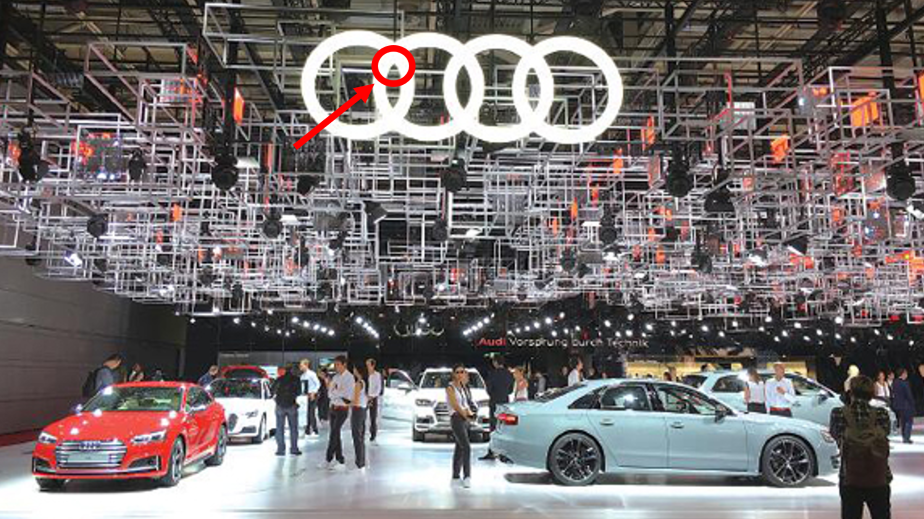
\includegraphics[width=0.9\linewidth]{audi.png}
		\caption{}
		\label{subfig:audi}
	\end{subfigure}%
	\begin{subfigure}[b]{.5\textwidth}
		\centering
		
\includegraphics[width=0.9\linewidth]{chanel.png}
		\caption{}
		\label{subfig:chanel}
	\end{subfigure}
	\begin{subfigure}[b]{.5\textwidth}
		\centering
		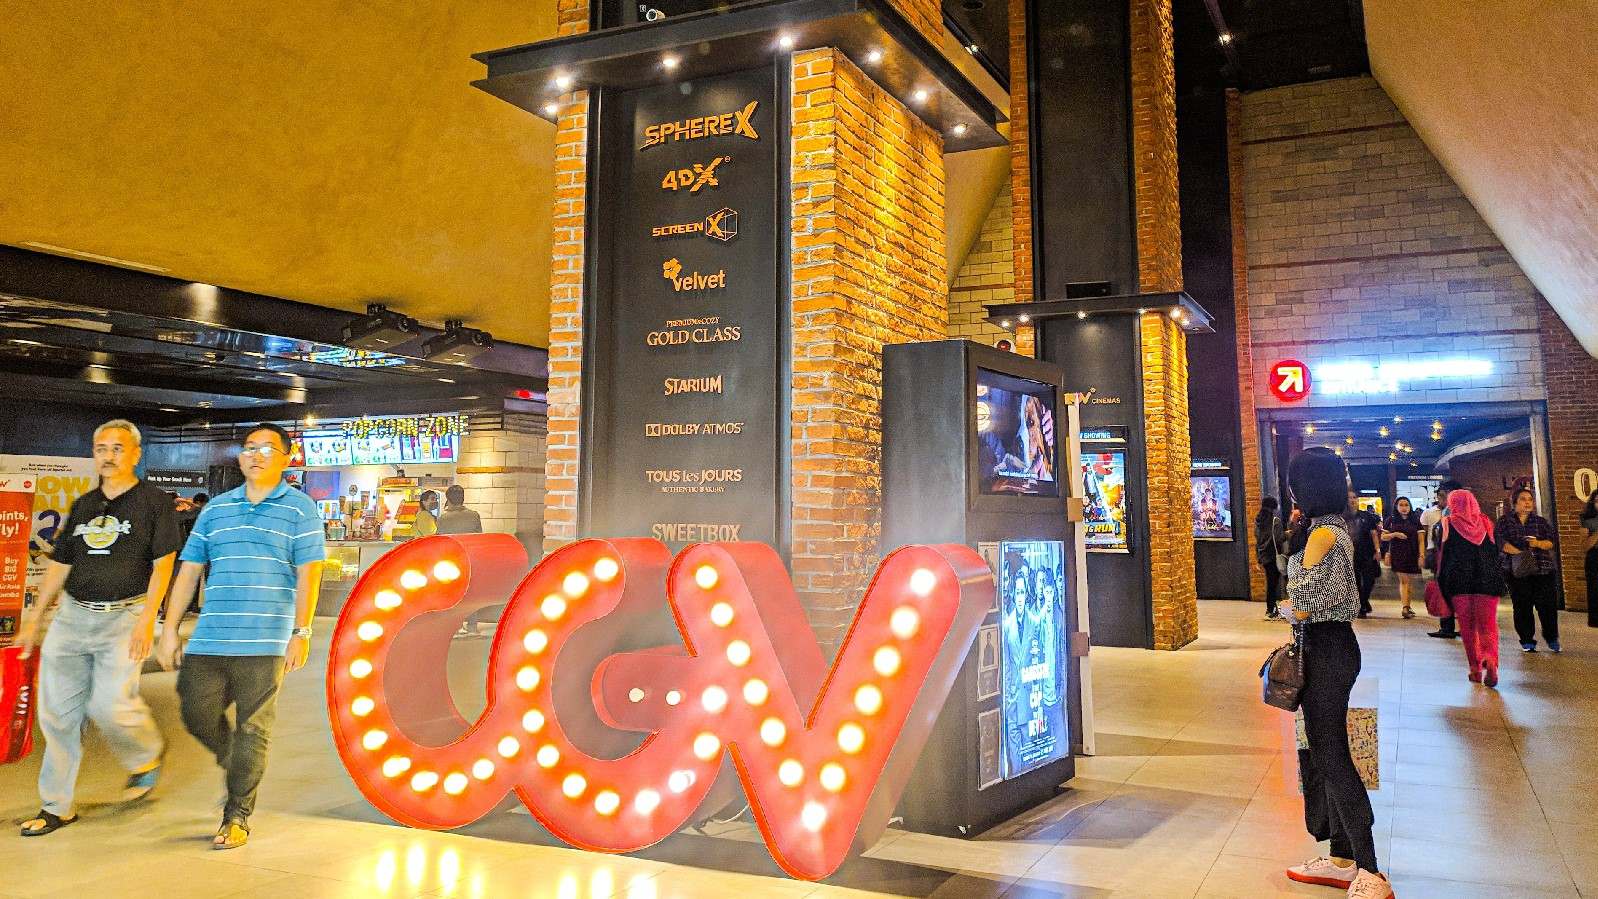
\includegraphics[width=0.9\linewidth]{cgv.jpg}
		\caption{}
		\label{subfig:cgv}
	\end{subfigure}%
	\begin{subfigure}[b]{.5\textwidth}
		\centering
		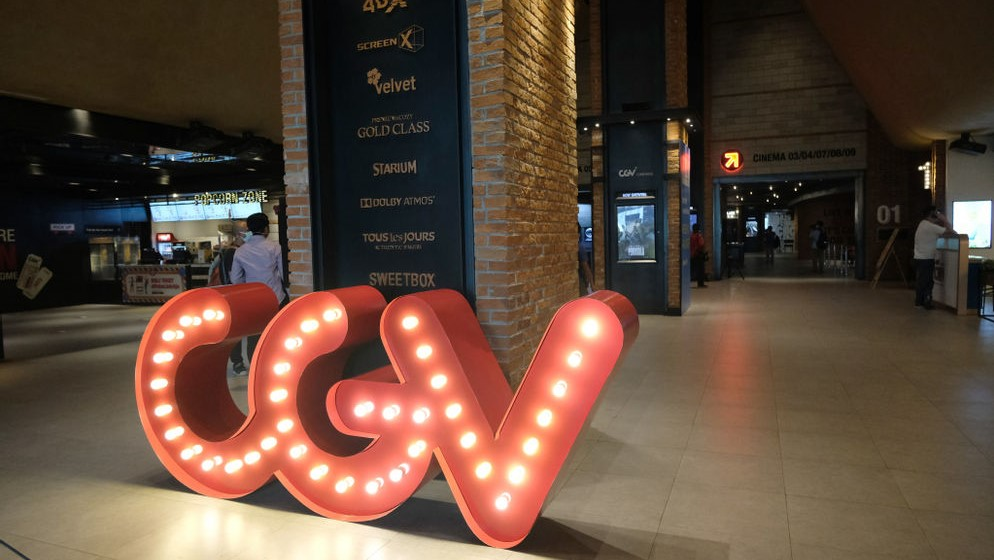
\includegraphics[width=0.9\linewidth]{cgv2.jpg}
		\caption{}
		\label{subfig:cgv2}
	\end{subfigure}
	\caption{Empat gambar di atas menunjukkan permasalahan yang dihadapi pada penelitian ini. Gambar (a) dan (b) merupakan gambar dari dua POI yang berbeda tetapi memiliki logo dengan bagian sudut yang mirip, sudut yang mirip tersebut kemungkinan akan menghasilkan fitur lokal yang mirip juga. Sedangkan pada gambar (c) dan (d) merupakan dua gambar dari POI yang sama tetapi banyak objek latar yang berbeda sehingga akan memunculkan fitur lokal yang tidak konsisten.}
	\label{fig:keypoint_non_unique}
\end{figure}
Fitur-fitur lokal yang tidak unik dan tidak konsisten tersebut akan dipisahkan dengan menggunakan metode \textit{clustering}. Metode \textit{clustering} merupakan teknik pemrosesan data yang akan mengelompokkan data-data dengan sifat yang mirip ke dalam satu kelompok. Metode \textit{clustering} pada penelitian ini akan menggunakan metode \textit{Agglomerative} dan DBSCAN. Penelitian ini mengasumsikan fitur lokal yang merepresentasikan suatu POI adalah fitur lokal yang muncul secara konsisten di gambar POI tersebut dan relatif unik terhadap POI tersebut.

\section{Rumusan Masalah}
\label{sec:rumusan}
Skripsi ini memiliki rumusan masalah sebagai berikut:
\begin{itemize}
	\item Bagaimana membuat model pengenalan POI berdasarkan fitur lokalnya menggunakan teknik \textit{data mining}?
	\item Bagaimana mengidentifikasi POI dalam sebuah gambar berisi POI dengan memanfaatkan model pengenalan POI yang telah dibuat?
\end{itemize}

\section{Tujuan}
\label{sec:tujuan}
Skripsi ini memiliki tujuan sebagai berikut:
\begin{itemize}
	\item Membuat perangkat lunak yang akan menghasilkan model pengenalan POI berdasarkan dari \textit{dataset} yang diberikan
	\item Membuat perangkat lunak yang dapat melakukan identifikasi POI dari sebuah gambar POI dengan menggunakan model yang dihasilkan.
\end{itemize}

\section{Batasan Masalah}
\label{sec:batasan}
Berikut batasan-batasan masalah dari skripsi ini:
\begin{itemize}
	\item Pengambilan fitur lokal untuk analisis dilakukan menggunakan metode SIFT dan ORB dengan implementasi OpenCV pada Python.
\end{itemize}

\section{Metodologi}
\label{sec:metlit}
Skripsi ini akan memiliki metodologi sebagai berikut:
\begin{enumerate}
	\item Melakukan studi literatur tentang metode OIR, teknik ekstraksi fitur lokal SIFT dan ORB, serta teknik-teknik \textit{data mining} yang digunakan pada skripsi ini. Studi literatur dilakukan dengan mencari dan membaca \textit{paper} atau buku yang berkaitan dengan topik tersebut.
	\item Mengumpulkan \textit{dataset} gambar POI yang diperlukan untuk penelitian dan pembuatan model identifikasi.
	\item Melakukan analisis pada latar belakang masalah pengenalan POI, dengan melihat sifat-sifat fitur lokal pada gambar POI.
	\item Menyusun rancangan perangkat lunak.
	\item Melakukan implementasi perangkat lunak.
	\item Menguji kinerja perangkat lunak.
	\item Menulis buku skripsi.
\end{enumerate}

\section{Sistematika Pembahasan}
\label{sec:sispem}
Sistematika pembahasan yang digunakan pada penelitian ini adalah sebagai berikut:
\begin{enumerate}
	\item Bab 1 Pendahuluan \\
	Bab ini berisi tentang hal-hal yang menggambarkan skripsi ini secara garis besar. Hal yang dibahas merupakan latar belakang masalah, rumusan masalah, tujuan penelitian, batasan masalah, dan metodologi penelitian.
	\item Bab 2 Landasan Teori \\
	Bab ini berisi tentang dasar-dasar teori dari teknik atau metode yang digunakan dalam skripsi ini, yaitu POI, OIR, metode SIFT, metode ORB, \textit{Best Score Increasing Subsequence} (BSIS), KD-Tree, teknik \textit{clustering} \textit{Agglomerative} dan DBSCAN, serta metode SIFT dan ORB di \textit{library} OpenCV.
	\item Bab 3 Analisis \\
	Bab ini berisi analisis pada masalah yang dibahas pada skripsi beserta solusi yang digunakan untuk menyelesaikan masalah tersebut.
	\item Bab 4 Perancangan \\
	Bab ini berisi tentang perancangan baik dari metode \textit{clustering} pada pemilihan fitur dan perancangan metode identifikasi POI dengan OIR. Bab juga akan berisi rancangan struktur \textit{file} dan \textit{folder} pada hasil akhir perangkat lunak.
	\item Bab 5 Implementasi dan Pengujian \\
	Bab ini berisi implementasi perangkat lunak pada metode pemilihan fitur dan identifikasi POI serta pengujian terhadap kinerja kedua metode tersebut.
	\item Bab 6 Kesimpulan dan Saran \\
	Bab ini berisi kesimpulan yang didapatkan dari hasil analisis serta keseluruhan implementasi dan pengujian yang dilakukan pada penelitian ini.
\end{enumerate}